\documentclass[10pt]{article}
\usepackage{color}
\usepackage{amsmath}
\usepackage{amssymb}
\usepackage{amsthm}
%\usepackage{amsrefs}
\usepackage{dsfont}
\usepackage{mathrsfs}
\usepackage{graphicx}
\usepackage{stmaryrd}
\usepackage{enumerate}
\usepackage[all]{xy}
\usepackage[mathcal]{eucal}
\usepackage{listings}
\usepackage{float}
\usepackage[margin = 1.5 in]{geometry}
\newcommand{\vect}[1]{\boldsymbol{#1}}
\usepackage{verbatim}  %%includes comment environment
\usepackage{subcaption}
\graphicspath{ {images/} }

%%Edit Here
\title{CMSC 25050 Computer Vision Project Report}
\author{Liu Cao \& Deqing Fu}
\date{}
\linespread{1.0}
\newtheorem{theorem}{Theorem} % PS
\newtheorem{question}{Question}
\newtheorem{lemma}[theorem]{Lemma}
\usepackage{tikz}
\usepackage{stmaryrd}
\usetikzlibrary{arrows}
\makeatletter
\newenvironment{solution}[1][\solutionname]{\par
  \pushQED{\qed}%
  \normalfont \topsep6\p@\@plus6\p@\relax
  \trivlist
%<amsbook|amsproc>  \itemindent\normalparindent
  \item[\hskip\labelsep
%<amsbook|amsproc>        \scshape
%<amsart|amsthm>        \itshape
\itshape 
    #1\@addpunct{.}]\ignorespaces
}{%
  \popQED\endtrivlist\@endpefalse
}
%    \end{macrocode}
%    Default for \cn{proofname}:
%    \begin{macrocode}
\providecommand{\solutionname}{Solution}

\makeatletter
\newcommand*{\indep}{%
  \mathbin{%
    \mathpalette{\@indep}{}%
  }%
}
\newcommand*{\nindep}{%
  \mathbin{%                   % The final symbol is a binary math operator
    %\mathpalette{\@indep}{\not}% \mathpalette helps for the adaptation
    \mathpalette{\@indep}{/}%
                               % of the symbol to the different math styles.
  }%
}
\setlength\parindent{24pt}
\newcommand*{\@indep}[2]{%
  % #1: math style
  % #2: empty or \not
  \sbox0{$#1\perp\m@th$}%        box 0 contains \perp symbol
  \sbox2{$#1=$}%                 box 2 for the height of =
  \sbox4{$#1\vcenter{}$}%        box 4 for the height of the math axis
  \rlap{\copy0}%                 first \perp
  \dimen@=\dimexpr\ht2-\ht4-.2pt\relax
      % The equals symbol is centered around the math axis.
      % The following equations are used to calculate the
      % right shift of the second \perp:
      % [1] ht(equals) - ht(math_axis) = line_width + 0.5 gap
      % [2] right_shift(second_perp) = line_width + gap
      % The line width is approximated by the default line width of 0.4pt
  \kern\dimen@
  \ifx\\#2\\%
  \else
    \hbox to \wd2{\hss$#1#2\m@th$\hss}%
    \kern-\wd2 %
  \fi
  \kern\dimen@
  \copy0 %                       second \perp
}
\usepackage{indentfirst}
\makeatother
\newcommand{\argmax}{\operatornamewithlimits{argmax}}
\newcommand{\argmin}{\operatornamewithlimits{argmin}}
\usepackage{algpseudocode}
\usepackage{algorithm}
\usepackage{bbm}
\usepackage{dsfont}
%Main
\begin{document}
\maketitle
\section*{Introduction}

 It's always amazing that living creatures have the ability to measure distance and reconstruct three-dimensional structures through the images they sense from their retina are in fact 2D. Then it brought up the question --- is there a way to reconstruct back the 3D structure from a set of images? Then the topic of "Structure from Motion" (SfM) arises. It has its profound influence in nearly every field, such as geoscience where scientists can utilize SfM to reconstruct and analyze terrains, and such as archaeology where archaeologists can use SfM to reconstruct lost ancient objects with their remaining documents of images. The most interesting is a gigantic project that reconstructs Rome using hundreds of thousands of images[1][2]. Attracted by these huge applications and research projects, we decided to learn and implement a simple \emph{Structure from Motion} model where we can deal with descent datasets. The pinhole camera model is used in our project.

In the project, we consider mainly two different scenarios that can happen in real life. One is that we only have a set of images and the intrinsic parameters of the camera and the other is that we have the set of images together with corresponding extrinsic parameters of each image. The latter would give us information of rotation matrix and the translation matrix of each image, while for the former we resorted to estimation of fundamental matrix and essential matrix to get such information.

We implemented triangulation to find the 3D location of matched feature points by choosing the point whose distance is the minimum to two matched beams from their camera locations and we ended up with a set of points in the 3D space, which is the cloud of the structure we want to reconstruct.

In terms of the data, we use the dinosaur dataset provided by University of Oxford Visual Geometry Group[3] which provides us the projection matrix $P = K [R\mid t]$, where $K$ is the intrinsic matrix, $R$ the rotation matrix and $t$ the translation matrix. While for the same dataset, we also assumes that we don't have the rotation and translation matrix ready and opt to estimate it from fundamental matrix as well.

The results of our project are the reconstructed 3D points cloud from the set of 2D images. The 2-frame reconstructed points cloud sees moderate success, but the multi-view reconstruction have a long way to go and we will propose several methods of future improvement to our implementation in the discussion section.


\section*{Method}

We firstly consider the scenario where the projection matrix $P= K [R\mid t]$ is given. 
Notice that for this kind of problem, $P \in \mathbb{R}^{3 \times 4}$, then we can write it as $P = [A \mid d]$.
Then we use the following decomposition method: firstly we use the QR algorithm to decompose P to get $A = qr$ where $q$ is orthogonal and $r$ is upper triangular. Then we have $$R = \begin{cases}
	q^{-1} & \text{ if } \det(q^{-1})  > 0 \\
	-q^{-1} & \text{ if } \det(q^{-1})  < 0 
\end{cases}$$
And we derive the intrinsic matrix as $K = r^{-1}$ and the translation matrix as $t = rb$. 

If we only have the intrinsic parameter of the camera while the extrinsic matrix of each image is not given, we can apply feature detection and matching first. In our implementation, we used SIFT feature detector and applied Distance Ratio Test (with a threshold of 1.25) to rule out false positive matching. We then use RANSAC method to find the \emph{fundamental matrix} from the matched points which is provided by the OpenCV library. Then we can derive \emph{essential matrix} from the fundamental matrix and the intrinsic camera parameter, and apply Single Value Decomposition on the essential matrix to compute the translation and rotation matrix, as Essential matrix is the product of the two. Among the 4 possible decomposition, only one of them projects points in front of both cameras, so we apply this test and remove this ambiguity. Note that we can now compute the camera center location ready for reconstruction. Let $c$ be the camera center, then we have $t = -Rc$. As rotation matrices are orthogonal matrices, then $R^{-1} = R^T$, thus we can compute the camera center from the extrinsic matrix as $c = - R^T \cdot t$. 


Please Refer to the Flow Chart for our methodology flow on page 3.

We referred to the textbook[4] for triangulation mentioned in the above flow chart. Essentially, all steps beforehand aims to get the rotation matrix and translation matrix for each image:
\begin{enumerate}[\qquad \quad 1.]
	\item Find Extrinsic Matrix $[R \mid t]$ for each image.
	\item For images $i$ and $i+1$, find their matched points $X_1$ and $X_2$, and find their camera centers $\vec{c}_1$ and $\vec{c}_2$. Then for each matched point pair $(\vec{x}_1, \vec{x}_2)$, we compute the direction vectors $\hat{v}_1 = \dfrac{\vec{c}_1 - \vec{x}_1}{||\vec{c}_1 - \vec{x}_1||}$ and $\hat{v}_2 = \dfrac{\vec{c}_2 - \vec{x}_2}{||\vec{c}_2 - \vec{x}_2||}$. Then we have two beams, whose parametrization are $\vec{b_1}(t) = \vec{x}_1 + \hat{v}_1 \cdot t$  and $\vec{b_2} (t) = \vec{x}_2 + \hat{v}_2 \cdot t$. Then we want to find a 3D point $\vec{p}$ whose distance to $\vec{b_1}$ and $\vec{b}_2$ achieves minimum. Then we can use the formula from the book (suppose the vectors are represented as column vectors) : $$\displaystyle \vec{p} = \left(\sum_{i=1}^2 (I - \hat{v}_i \hat{v}_i^T ) \right)^{-1} \cdot \left(\sum_{i=1}^2 (I - \hat{v}_i \hat{v}_i^T ) \vec{c}_i \right)$$
\end{enumerate}

Thus we derive a set of $\vec{p}$'s, which is the cloud of points of our reconstruction. 

\begin{figure}[H]
    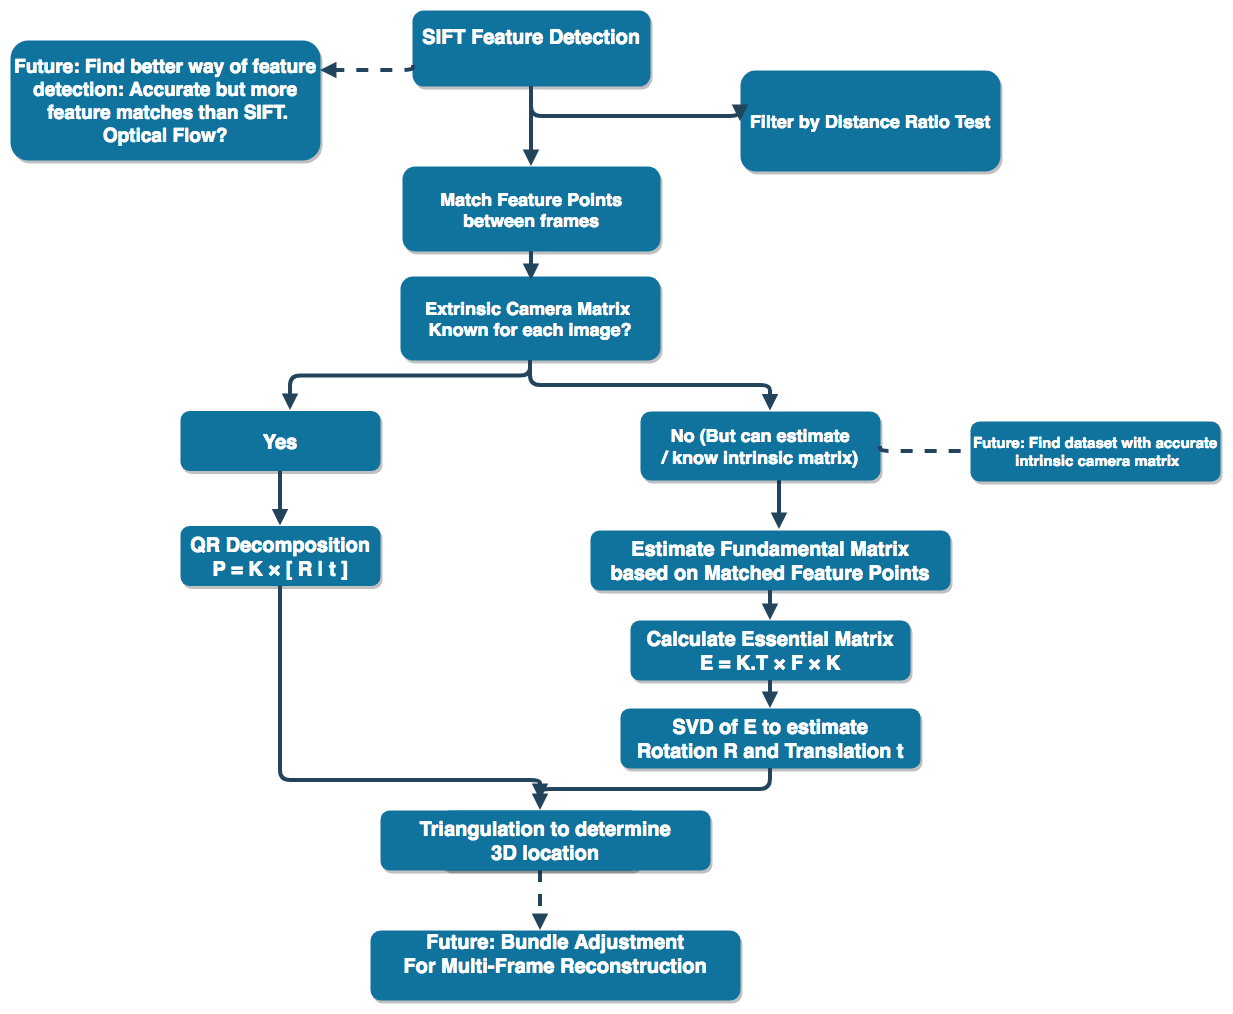
\includegraphics[width=1.2\linewidth]{Diagram.png}
  \caption{Structure from Motion Algorithm and Procedure}
  \label{fig:procedure}
\end{figure}

\newpage
\section*{Experimental Results}
Below is the 2-frame reconstructed 3D point cloud of the dinosaur dataset. At first glance, this is an acceptable result as we can see the structure of dinosaur hands, legs and tails very obviously.


\begin{figure}[h!]
  \centering
  \begin{subfigure}[h!]{0.7\linewidth}
    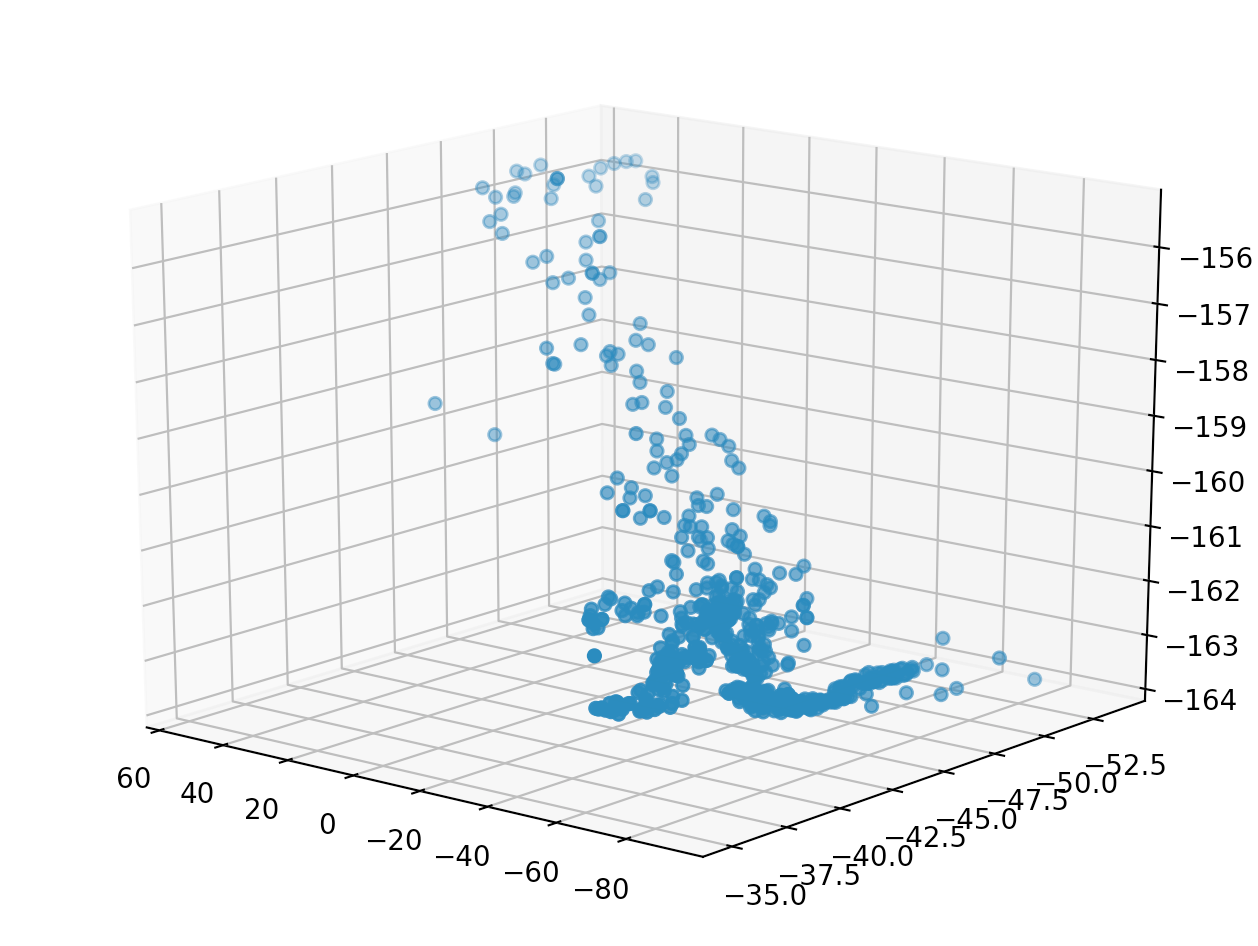
\includegraphics[width=\linewidth]{cloud.jpg}
    \caption{Reconstructed 3D point cloud of the dinosaur.}
  \end{subfigure}
  \begin{subfigure}[h!]{0.5\linewidth}
    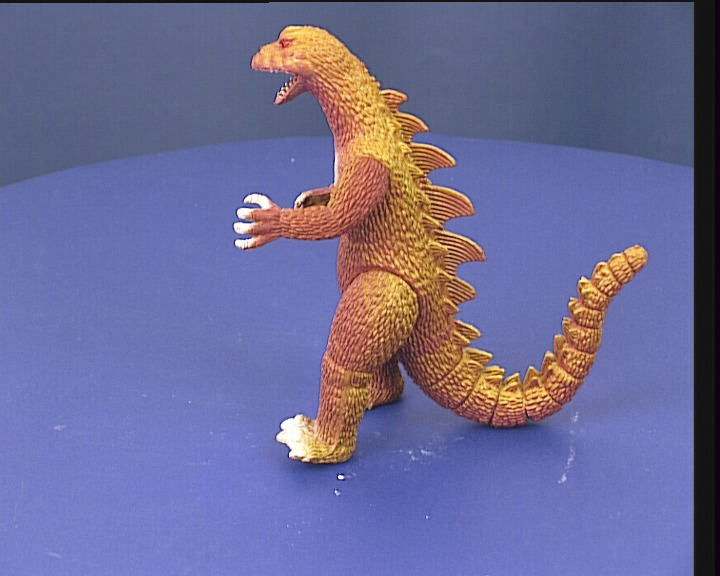
\includegraphics[width=\linewidth]{original.jpg}
    \caption{Dinosaur Photo}
  \end{subfigure}
  \caption{2-Frame SFM Reconstruction of Dinosaur}
  \label{fig:coffee}
\end{figure}

Our reference result from the decomposed projection matrix provided by the dataset has a flaw in the accuracy of the QR decomposition and thus does not look very good.

To qualitatively estimate the quality of our 3D point cloud reconstruction, we project the reconstruction 3D cloud points to every 2D images; And among those 3D points that have corresponding 2D feature points in a specific image, we add the square of Euclidean distances (between the projection point and the feature point) together then take the square root of the total sum. Note that for each image there are a different number of the square of distance added to the total due to the different number of features and matched projected 3D points.

For our 2-frame reconstruction of the dinosaur dataset without knowing extrinsic camera matrix, this yields a value of approximately 725, while if adding more frames to the reconstruction will simply blow this value up by tens (or even more of many frames are added) of times due to error accumulation. Admittedly, the result is not very good, as there are multiple ways we can improve our implementation but didn't have the chance to do so due to time constraint. We will talk about them in the next section.


\section*{Discussion}

There are many possible future improvements to our implementation that we would like to try should time permit: ① Implementing Bundle Adjustment, ② using a better Matching Procedure and ③ use a better method to calibrate the intrinsic camera (or find a method of reconstruction less prone to the error in the estimated value). 

\begin{enumerate}

\item Implementing Bundle Adjustment
Bundle Adjustment would give our implementation a direct upgrade in terms of accuracy for multi-frame reconstruction. 

By taking in a list of cloud points, camera translation matrices and rotation matrices, and intrinsic camera matrices, bundle adjustment would refine each new cloud point by performing robust non-linear minimization of the measurement (re-projection) errors.[book 7.4] (error defined as between the image locations of observed and predicted image points)

\item Feature Detection and Matching Procedure 
In our submitted version, we employed the SIFT feature detector with distance ratio test. There are other options we ruled out, such as ORB as the feature detector or nearest neighbor as the matching method, as we only want features with good qualities so we can lower the number of false matchings. However, in our own implementation that stems from the homework 2 SIFT-like feature detector and matching with distance ratio test, we ended up with too few matched features although we usually maintain a matching accuracy around 90\%. Essentially, our implementation has us consider the tradeoff between whether we can eliminate enough false positives to maintain accuracy and whether we have enough number of matched feature points. We switched to OpenCV library's well-written SIFT detector to have a larger number of matched points with slightly lower accuracy. (The program submitted have options to switch between ours and OpenCV's, and the above result in section III used OpenCV library.)

Nonetheless, the number of matched points is far less than what ORB detector would offer and we imagine there could be a better way to do this, especially in the case of 360-degree reconstruction. The literature points to Optical Flow [5], among other possibilities and this will be a future topic to explore.

\item Calibration the intrinsic camera
One struggle we had throughout our implementation is due to the fact that our dataset does not have an explicitly defined intrinsic camera matrix. We used QR decomposition to extract the intrinsic camera matrix from the projection matrix, and the estimated focal length have a non-negligible error. A good future step would be to try taking photos ourselves with a well-calibrated camera.
\end{enumerate}

We are having issues uploading photos and repositories to canvas so only a minimal version is provided. Please refer to our Github Repo for the full code: 
https://github.com/CTCC1/simple-SfM 

\section*{Reference}

[1] Sameer Agarwal, Noah Snavely, Ian Simon, Steven M. Seitz and Richard Szeliski, "Building Rome in a Day" in International Conference on Computer Vision, 2009, Kyoto, Japan.

[2] Sameer Agarwal, Yasutaka Furukawa, Noah Snavely, Brian Curless, Steven M. Seitz and Richard Szeliski, "Reconstructing Rome", in IEEE Computer, pp. 40-47, June, 2010 

[3]http://www.robots.ox.ac.uk/~vgg/data/data-mview.html
Dataset of Visual Geometry Group, Department of Engineering Science, University of Oxford

[4]Richard Szeliski, Computer Vision: Algorithms and Applications, Chapter 7

[5]T. Brox and J. Malik, "Large Displacement Optical Flow: Descriptor Matching in Variational Motion Estimation," in IEEE Transactions on Pattern Analysis and Machine Intelligence, vol. 33, no. 3, pp. 500-513, March 2011.


\end{document} 